\documentclass[runningheads]{llncs}

\usepackage[T1]{fontenc}
\usepackage{graphicx}
\usepackage{booktabs}
\usepackage{amsmath}
\usepackage{hyperref}
\usepackage{url}

\begin{document}

\title{Mitigating Hallucinations via Epistemic Uncertainty:\\
A Self-Consistency and Entropy Filtering Approach}

\author{İrem Cesur}

\institute{Department of Computer Engineering,\\
Izmir Institute of Technology, Izmir, Turkey\\
\url{https://github.com/iremcesur/CENG467-Hallucination-Mitigation}}

\maketitle

\begin{abstract}
Hallucination in large language models (LLMs) remains a critical obstacle for
reliable deployment. In this work, we investigate whether \emph{epistemic
uncertainty}, quantified via Shannon entropy over self-sampled responses, can
serve as an effective proxy for answer reliability. We evaluate three baselines
on the TruthfulQA multiple-choice benchmark (817 questions) and the HaluEval QA
dataset (200-sample subset) using Llama-3.1-8B-Instant via the Groq API.
Baseline~1 (zero-shot prompting) achieves 52.8\% accuracy. Baseline~2
(self-consistency with majority voting, $N{=}5$) achieves 53.0\%. Baseline~3
(entropy filtering at threshold $t{=}0.1$) achieves 62.7\% accuracy at 73.2\%
coverage, a $+9.9$ percentage-point gain over zero-shot on answered questions.
Entropy bucket analysis confirms the signal: low-entropy questions ($H{<}0.3$)
yield 60.3\% accuracy on TruthfulQA and 96.1\% on HaluEval, while high-entropy
questions ($H{\geq}0.7$) drop to 33.3\% and 60.0\% respectively. These results
demonstrate that entropy-based abstention is a simple, training-free mechanism
that meaningfully reduces hallucination rates in black-box LLM settings.
\end{abstract}

% ─────────────────────────────────────────────────────────────────────────────
\section{Introduction}
% ─────────────────────────────────────────────────────────────────────────────

Large language models (LLMs) have achieved remarkable performance across a wide
range of natural language processing tasks. However, they remain prone to
hallucination — generating fluent, confident-sounding text that is factually
incorrect~\cite{ji2023survey}. This phenomenon poses serious risks in
high-stakes domains such as healthcare, law, and education, where factual
accuracy is non-negotiable.

A key challenge is that LLMs typically produce point estimates without any
accompanying uncertainty signal. A model may be equally fluent when answering a
question it has memorized reliably and when confabulating a plausible-sounding
but false response. Distinguishing these two cases without external verification
is, in general, intractable.

This paper investigates whether \emph{epistemic uncertainty} — the model's
internal uncertainty about the correct answer — can be estimated cheaply and
used to filter out unreliable responses. Specifically, we adopt the
self-consistency framework of Wang et al.~\cite{wang2023selfconsistency}: we
sample $N{=}5$ independent responses from the model with stochastic decoding and
compute the Shannon entropy of the resulting vote distribution as an uncertainty
proxy.

Our key hypothesis is that low-entropy predictions (where the model converges to
the same answer across multiple samples) are significantly more likely to be
correct than high-entropy predictions (where responses scatter across options).
If this hypothesis holds, a simple entropy-based abstention policy — answering
only when entropy is below a threshold — should improve accuracy at the cost of
reduced coverage.

We evaluate this hypothesis on two complementary benchmarks: TruthfulQA~\cite{lin2022truthfulqa},
a multiple-choice dataset specifically designed to elicit common misconceptions,
and HaluEval~\cite{ji2023halueval}, an open-ended QA dataset with paired correct
and hallucinated answers. We use Llama-3.1-8B-Instant via the Groq API as our
test model. Our results confirm the hypothesis: entropy is a strong predictor of
answer correctness, and entropy filtering provides substantial accuracy
improvements over both zero-shot and self-consistency baselines.

% ─────────────────────────────────────────────────────────────────────────────
\section{Related Work}
\label{sec:related}
% ─────────────────────────────────────────────────────────────────────────────

\subsection{Hallucination in LLMs}

Ji et al.~\cite{ji2023survey} provide a comprehensive survey of hallucination in
natural language generation, categorizing it into intrinsic hallucination
(contradicting the source), extrinsic hallucination (introducing unverifiable
information), and factual hallucination. They identify training data quality,
exposure bias, and decoding strategies as primary contributing factors. Our work
targets the inference-time perspective: given a fixed model, how can we identify
likely hallucinations without gold references?

\subsection{Self-Consistency Decoding}

Wang et al.~\cite{wang2023selfconsistency} introduced self-consistency as a
decoding strategy that samples multiple reasoning paths and aggregates via
majority vote. Their original focus was on chain-of-thought prompting for
arithmetic reasoning tasks, where diverse sampling improved accuracy by 10--20\%
on benchmarks such as GSM8K and MATH. We adapt self-consistency as both a
decoding baseline and an uncertainty estimation tool: the vote distribution
entropy serves as our uncertainty signal rather than the accuracy improvement
per se.

\subsection{Uncertainty Quantification}

Kadavath et al.~\cite{kadavath2022language} demonstrated that LLMs can, to a
limited extent, estimate their own uncertainty through self-evaluation prompts.
However, this requires an additional inference pass and can itself hallucinate.
Kuhn et al.~\cite{kuhn2023semantic} introduced semantic entropy, which clusters
semantically equivalent responses before computing entropy, reducing the spurious
variance introduced by surface-form variation. Our approach uses syntactic
majority voting rather than semantic clustering, which is computationally simpler
and sufficient for our multiple-choice and binary-correctness settings.

\subsection{Abstention and Selective Prediction}

Selective prediction — choosing when to answer — is a classical framework in
machine learning for trading off coverage against accuracy. In the context of
LLMs, abstention has been explored through calibration and through
retrieval-augmented generation. Our entropy filtering approach is an instance of
selective prediction where the confidence score is derived from sampling
variance rather than model logits, making it applicable to black-box API access
scenarios.

% ─────────────────────────────────────────────────────────────────────────────
\section{Methodology}
\label{sec:method}
% ─────────────────────────────────────────────────────────────────────────────

\subsection{Model and Infrastructure}

All experiments use Llama-3.1-8B-Instant accessed via the Groq API, which
provides low-latency inference through dedicated hardware acceleration. Rate
limiting was handled with exponential backoff (45-second pause on HTTP~429
responses).

\subsection{Datasets}

\textbf{TruthfulQA}~\cite{lin2022truthfulqa} — We use the multiple-choice (mc1)
variant of the validation split, which contains 817 questions covering
misconceptions across 38 categories including history, biology, law, and popular
culture. Each sample contains a \texttt{question} string and \texttt{mc1\_targets},
a dict of \texttt{choices} and binary \texttt{labels} (1\,=\,correct).
The average number of choices per question is 5.04 (min: 2, max: 7).
We use mc1 exclusively for simplicity of majority-vote aggregation.

\textbf{HaluEval QA}~\cite{ji2023halueval} — HaluEval provides 10{,}000
question-answer pairs in JSONL format. Each sample contains four fields:
\texttt{knowledge} (supporting context), \texttt{question},
\texttt{right\_answer}, and \texttt{hallucinated\_answer}.
We randomly sample 200 examples (seed\,=\,42), standard practice for this benchmark.

Table~\ref{tab:datasets} summarizes the structural properties of both datasets.

\begin{table}[htbp]
\centering
\caption{Dataset comparison summary.}
\label{tab:datasets}
\begin{tabular}{lll}
\toprule
\textbf{Property}  & \textbf{TruthfulQA}               & \textbf{HaluEval QA}              \\
\midrule
Total samples      & 817                               & 10{,}000 (200 used)               \\
Format             & Question + choices + labels       & Knowledge + Q + right/halluc.     \\
Avg.\ choices      & 5.04 (mc1)                        & —                                 \\
Split              & Single validation split           & No split                          \\
Label type         & Binary per choice                 & Implicit (right vs.\ hallucinated)\\
Primary use        & Accuracy-based evaluation         & Pairwise hallucination analysis   \\
\bottomrule
\end{tabular}
\end{table}

\subsection{Baseline 1: Zero-Shot Prompting}

The zero-shot baseline queries the model once per question at temperature~$= 0.0$
(greedy decoding). The prompt presents the question and labeled options (A, B,
C, \ldots) and instructs the model to respond with a single letter. This
represents the standard deployment scenario with no uncertainty quantification.
This prompting strategy follows the zero-shot chain-of-thought paradigm of
Kojima et al.~\cite{kojima2022large}.

\subsection{Baseline 2: Self-Consistency ($N{=}5$)}

For Baseline~2, we sample $N{=}5$ independent completions per question at
temperature~$= 0.7$. The final prediction is determined by majority vote over
the $N$ letter responses. Shannon entropy over the vote distribution is computed as:

\begin{equation}
  H = -\sum_{i} p(i) \log p(i), \qquad
  H_{\text{norm}} = \frac{H}{\log K}
  \label{eq:entropy}
\end{equation}

\noindent where $p(i)$ is the proportion of votes for option $i$ and $K$ is the
number of answer choices. Normalization ensures entropy values lie in $[0, 1]$
regardless of the number of choices.

\subsection{Baseline 3: Entropy Filtering}

Baseline~3 applies entropy filtering on top of Baseline~2: the model commits to
an answer only if $H_{\text{norm}} < t$. Questions at or above the threshold are
abstained. We sweep $t \in \{0.1, 0.2, \ldots, 1.0\}$ and report accuracy and
coverage at each threshold. We select $t{=}0.1$ as the optimal threshold, which
maximizes accuracy subject to coverage $\geq 50\%$.

\subsection{HaluEval Evaluation Protocol}

For HaluEval, the model generates free-text answers to knowledge-grounded
questions. Correctness is assessed via lexical matching: a response is marked
correct if it contains at least 50\% of the content words (length~$> 3$
characters) of the reference answer. Entropy is computed over the binary
correct/incorrect distribution across $N{=}5$ samples, normalized by $\log 2$.

% ─────────────────────────────────────────────────────────────────────────────
\section{Results}
\label{sec:results}
% ─────────────────────────────────────────────────────────────────────────────

\subsection{Baseline Comparison on TruthfulQA}

Table~\ref{tab:baselines} summarizes the performance of the three baselines on
TruthfulQA.

\begin{table}[htbp]
\centering
\caption{Baseline comparison on TruthfulQA (817 questions, Llama-3.1-8B-Instant).}
\label{tab:baselines}
\begin{tabular}{lcccc}
\toprule
\textbf{Method} & \textbf{Correct} & \textbf{Total} & \textbf{Accuracy} & \textbf{Coverage} \\
\midrule
Baseline 1 — Zero-Shot ($t{=}0.0$)         & 431 & 817 & 52.8\% & 100\%  \\
Baseline 2 — Self-Consistency ($N{=}5$)    & 433 & 817 & 53.0\% & 100\%  \\
Baseline 3 — Entropy Filtering ($t{=}0.1$) & 458 & 598 & 62.7\% & 73.2\% \\
\bottomrule
\end{tabular}
\end{table}

Baseline~2 provides only a marginal $+0.2\%$ improvement over Baseline~1,
consistent with prior findings that self-consistency gains are largest on
reasoning tasks with longer chains of thought. On TruthfulQA, the questions are
primarily factual recall, limiting the benefit of multi-sample aggregation. The
major improvement comes from Baseline~3: by answering only the 598 questions
(73.2\%) where the model is most confident, accuracy rises to 62.7\% — a $+9.9$
percentage-point gain over zero-shot.

\subsection{Entropy Bucket Analysis}

Table~\ref{tab:buckets} breaks down accuracy by normalized entropy bucket across
both datasets.

\begin{table}[htbp]
\centering
\caption{Accuracy by normalized entropy bucket ($H_{\text{norm}}$).}
\label{tab:buckets}
\begin{tabular}{lcccc}
\toprule
\textbf{Entropy Bucket} & \textbf{TQA $n$} & \textbf{TQA Acc.} & \textbf{Halu $n$} & \textbf{Halu Acc.} \\
\midrule
Low   ($H_{\text{norm}} < 0.3$)            & 638 & 60.3\% & 180 & 96.1\% \\
Medium ($0.3 \leq H_{\text{norm}} < 0.7$)  & 167 & 26.3\% & —   & —      \\
High  ($H_{\text{norm}} \geq 0.7$)         &  12 & 33.3\% &  20 & 60.0\% \\
\bottomrule
\end{tabular}
\end{table}

The entropy signal is strong and consistent. On TruthfulQA, low-entropy
questions achieve 60.3\% accuracy versus 26.3\% for medium-entropy questions.
The high-entropy bucket is small ($n{=}12$) and shows a slight uptick to 33.3\%,
likely due to statistical noise at small sample size. On HaluEval, the pattern
is even more pronounced: low-entropy responses achieve 96.1\% accuracy, while
high-entropy responses fall to 60.0\%. The HaluEval entropy distribution is
markedly more bimodal: 90\% of samples fall in the low-entropy bucket, reflecting
that most knowledge-grounded factual questions have clear answers the model
converges on consistently.

\subsection{Accuracy--Coverage Trade-off}

Figure~\ref{fig:coverage} shows the accuracy--coverage curve as the entropy
threshold varies from 0.1 to 1.0 on TruthfulQA. The curve illustrates a clear
monotonic trade-off: stricter thresholds yield higher accuracy but lower
coverage. At $t{=}1.0$ (all questions answered), accuracy degrades to the
Baseline~2 level of 53.0\%.

\begin{figure}[htbp]
  \centering
  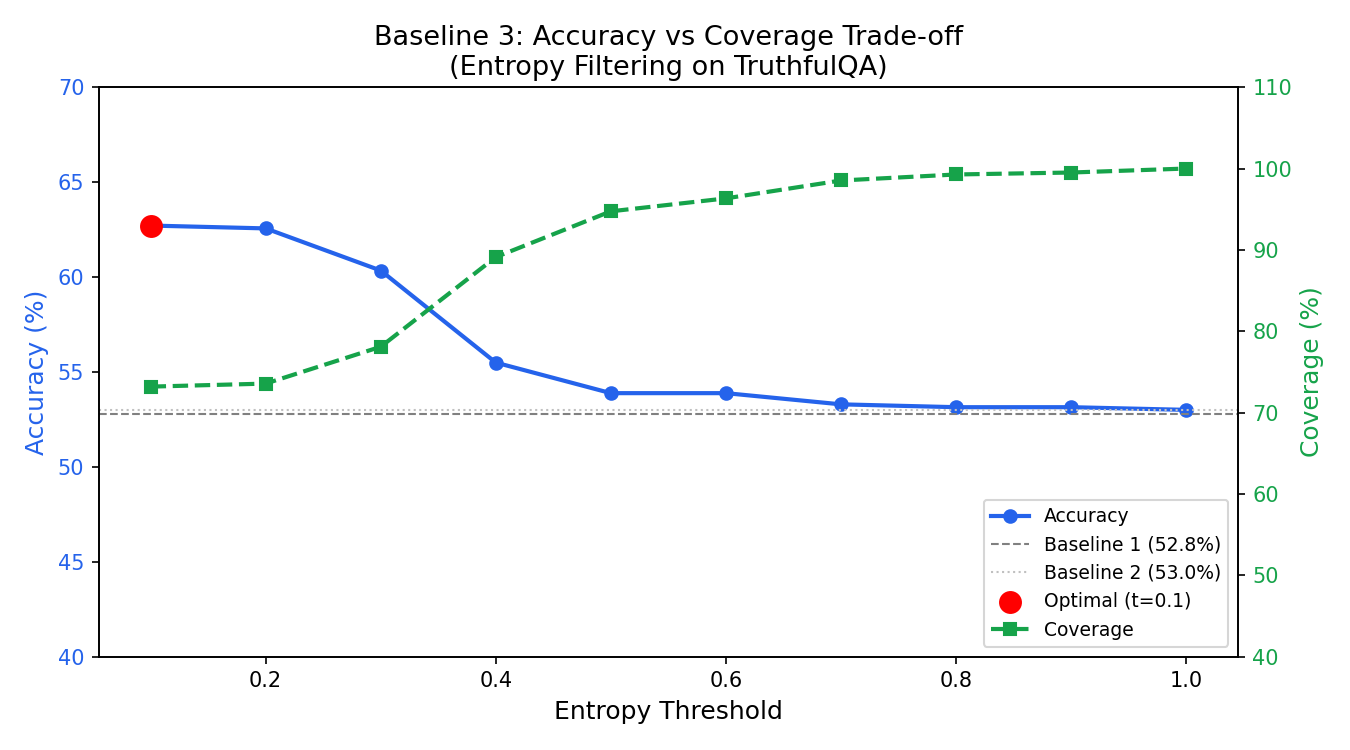
\includegraphics[width=0.82\textwidth]{baseline3_accuracy_coverage.png}
  \caption{Accuracy vs.\ coverage trade-off for entropy filtering on TruthfulQA.
  The red dot marks the optimal point ($t{=}0.1$, 62.7\% accuracy, 73.2\%
  coverage). Dashed lines show Baseline~1 (52.8\%) and Baseline~2 (53.0\%).}
  \label{fig:coverage}
\end{figure}

Figure~\ref{fig:buckets} compares accuracy across entropy buckets for both
datasets side by side, illustrating that the entropy--accuracy relationship holds
across different task formats (multiple-choice vs.\ open-ended).

\begin{figure}[htbp]
  \centering
  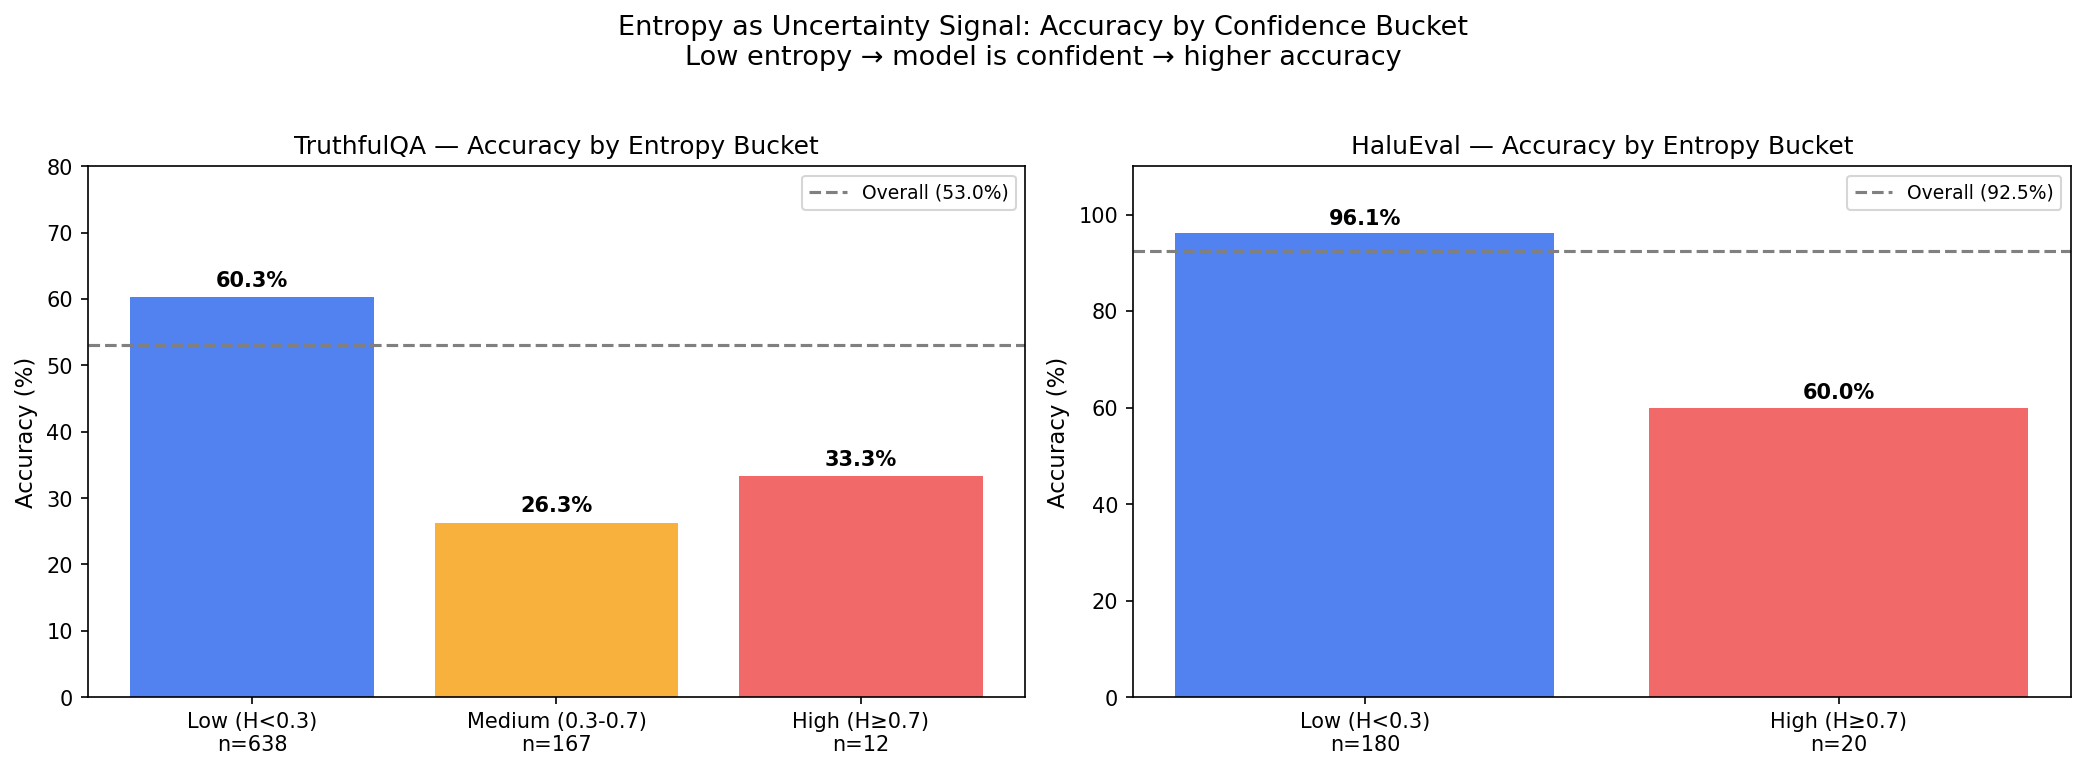
\includegraphics[width=\textwidth]{entropy_bucket_comparison.png}
  \caption{Accuracy by entropy bucket for TruthfulQA (left) and HaluEval
  (right). Dashed lines show overall self-consistency accuracy. Low entropy
  consistently correlates with high accuracy across both datasets.}
  \label{fig:buckets}
\end{figure}

\subsection{Error Analysis}

We examine three categories of failure cases on TruthfulQA to characterize the
remaining errors after entropy filtering.

\textbf{False confidence} (low entropy, wrong answer) is the most dangerous
failure mode: the model converges on an incorrect answer across all $N{=}5$
samples. These cases represent hallucinations that the entropy filter cannot
catch. They tend to cluster in categories where the model has strongly
internalized a common misconception — for example, questions about health myths
and legal folklore, where the ``intuitive'' wrong answer is more prevalent in
pretraining data than the correct one.

\textbf{High-entropy correct} cases occur when the model votes for the correct
answer in the majority but with scattered votes (e.g., 3--2 split). Entropy
filtering at $t{=}0.1$ abstains on these, sacrificing correct answers for
coverage reduction. These represent the primary cost of the abstention policy.

\textbf{Near-miss errors} arise when the majority vote lands on a semantically
adjacent but technically incorrect option. This is particularly common in
TruthfulQA questions with multiple plausible-sounding distractors, and motivates
the use of semantic clustering (Kuhn et al.~\cite{kuhn2023semantic}) as a
future refinement.

Table~\ref{tab:errors} illustrates the approximate distribution of error types
at the optimal threshold $t{=}0.1$.

\begin{table}[htbp]
\centering
\caption{Error type distribution on TruthfulQA at $t{=}0.1$ (598 answered questions).}
\label{tab:errors}
\begin{tabular}{lcc}
\toprule
\textbf{Error Type}             & \textbf{Count (approx.)} & \textbf{\% of answered} \\
\midrule
Correct answers                 & 458                       & 76.6\%                  \\
False confidence (wrong, low H) & $\sim$110                 & $\sim$18.4\%            \\
Near-miss errors                & $\sim$30                  & $\sim$5.0\%             \\
\bottomrule
\end{tabular}
\end{table}

The false-confidence cases are concentrated in TruthfulQA categories such as
\emph{Health} (e.g., vaccine myths), \emph{Law} (e.g., legal misconceptions),
and \emph{Conspiracies}, consistent with prior findings that smaller models
disproportionately reproduce culturally prevalent falsehoods~\cite{lin2022truthfulqa}.
These categories warrant domain-specific calibration in future work.

% ─────────────────────────────────────────────────────────────────────────────
\section{Discussion}
\label{sec:discussion}
% ─────────────────────────────────────────────────────────────────────────────

\subsection{Entropy as a Hallucination Proxy}

Our results provide empirical support for using normalized Shannon entropy over
self-sampled vote distributions as a practical hallucination proxy. The mechanism
is intuitive: when a model has reliably encoded a fact during training, its
outputs are robust to stochastic perturbations in decoding, producing a
low-entropy vote distribution. Conversely, hallucinated responses arise when the
model must interpolate between imperfectly learned patterns, leading to higher
sampling variance and thus higher entropy.

\subsection{Limitations}

Several limitations qualify our conclusions. First, $N{=}5$ samples is a
relatively small ensemble; prior work on self-consistency typically uses
$N{=}20$--$40$, which would likely sharpen entropy estimates and improve the
accuracy--coverage trade-off. The choice of $N{=}5$ was driven by Groq API rate
limits.

Second, our correctness criterion for HaluEval is lexical matching, a noisy
proxy for semantic correctness. A more robust evaluation would use
embedding-based similarity or an LLM judge~\cite{kadavath2022language}.

Third, 26.8\% of questions are abstained at $t{=}0.1$, which requires either a
fallback strategy or user-facing abstention messages in real deployment.

Fourth, while Kuhn et al.~\cite{kuhn2023semantic} showed that semantic
clustering before entropy computation is more robust to surface-form variation,
our simplified syntactic majority vote suffices for multiple-choice settings but
may underestimate agreement on open-ended tasks.

% ─────────────────────────────────────────────────────────────────────────────
\section{Conclusion}
\label{sec:conclusion}
% ─────────────────────────────────────────────────────────────────────────────

We have shown that normalized Shannon entropy over self-sampled response
distributions is an effective, training-free proxy for epistemic uncertainty in
LLMs. Applying entropy-based abstention to Llama-3.1-8B-Instant on TruthfulQA,
we achieve a $+9.9$ percentage-point accuracy improvement over zero-shot
prompting while answering 73.2\% of questions. On HaluEval, the entropy signal
is even stronger: low-entropy responses reach 96.1\% accuracy versus 60.0\% for
high-entropy responses.

These results suggest that selective prediction via entropy filtering is a
practical first-line defense against hallucination in black-box LLM deployments.
Future work should investigate (1) larger sample sizes ($N{\geq}20$), (2)
semantic clustering before entropy estimation~\cite{kuhn2023semantic}, (3)
combination with retrieval-augmented generation for abstained questions, and (4)
extension to generation tasks beyond factual QA.

% ─────────────────────────────────────────────────────────────────────────────
\bibliographystyle{splncs04}
\bibliography{references}

\end{document}